\documentclass{beamer}
\usepackage{mathrsfs}  
\usepackage{xcolor}
\usepackage{setspace}
\usepackage{comment}
\usepackage{lmodern}
\usepackage[utf8x]{inputenc}
\usepackage[T1]{fontenc}

% config du thgeme metropolis
\usetheme[progressbar=frametitle,block=fill, titleformat=smallcaps,sectionpage=progressbar,]{metropolis}



\title{Statistiques, Probabilités, Analyse Spatiale}
\subtitle{Présentation du Module}
\date{2021-2022}
\author{Paul Chapron \textsuperscript{1} \& Yann Ménéroux \textsuperscript{1} \& Juste Raimbault }
\institute{ \textsuperscript{1}IGN-ENSG-UGE}



%definition de la couleur du texte dans la balise \alert{}
\definecolor{vertIGN}{HTML}{96C31E} % vert IGN %vrai valeur #97BE0D
\setbeamercolor{alerted text}{fg=vertIGN}

\definecolor{grisIGN}{HTML}{22292F} % Gris IGN tiré vers le noir 
\setbeamercolor{background canvas}{bg=grisIGN}




% code pour placer le log ENSG dans le bandeau de titre 
\makeatletter
\setbeamertemplate{frametitle}{%
  \nointerlineskip%
  \begin{beamercolorbox}[%
      wd=\paperwidth,%
      sep=0pt,%
      leftskip=\metropolis@frametitle@padding,%
      rightskip=\metropolis@frametitle@padding,%
    ]{frametitle}%
  \metropolis@frametitlestrut@start%
  \insertframetitle%
  \nolinebreak%
  \metropolis@frametitlestrut@end%
  \hfill
  \raisebox{-0.6ex}{
\includegraphics[height=4ex,keepaspectratio]{img/logoENSG_small.jpg}}
  \end{beamercolorbox}%
}
\makeatother




% logo ENSG première page 
\titlegraphic{\vspace{4cm}\flushright
\includegraphics[width=2cm,height=2cm]{img/logoENSG_big.png}} 



\begin{document}
\metroset{background=dark} % change background theme according to manual
\maketitle	

\section{Introduction} 



\begin{frame}
\frametitle{Citations en vrac}

\begin{tiny}


\hfill «If you torture data long enough, it will confess» \\
\hfill Ronald Coase\\
\vfill
\hfill «It is a capital mistake to theorize before one has data.»\\
\hfill Sherlock Holmes\\
\vfill
\hfill «All models are wrong, but some are useful.»\\
\hfill  George Box\\
\vfill
\hfill «Data scientist (noun): Person who is better at statistics than any software engineer and better at software engineering than any statistician.»\\
\hfill Josh Wills\\
\vfill
\hfill «There are three kinds of falsehoods: lies, damned lies and statistics» \\
\hfill Mark Twain\\ 
\vfill

\hfill «Les statistiques sont une forme d'accomplissement de désir, tout comme les rêves.» \\
\hfill Jean Baudrillard\\
\vfill



\hfill «Ce qui est simple est faux, ce qui est compliqué est inutile.» \\
\hfill Paul Valéry\\
\vfill


\hfill «La statistique est la première des sciences inexactes.»\\
\hfill  Édouard et Jules de Goncourt



\end{tiny}


\end{frame}





\begin{frame}
\frametitle{Survol des trois thématiques}
\begin{itemize}
\item \alert{Statistique} : Démarche scientifique visant à acquérir des connaissances sur l'état d'un objet difficilement perceptible sur le plan cognitif : 
\begin{itemize}
\item objet \alert{massif} (population, big data...) : résumer, synthétiser, visualiser, échantillonner, compresser...
\item objet \alert{incertain} (observations bruitées) : moyenner, borner, encadrer, compenser... \newline \pause
\end{itemize}

En général, la statistique sert à  \alert{décrire} des états présents ou passés.


\end{itemize}
\end{frame}


\begin{frame}
\frametitle{Survol des trois thématiques}

\begin{itemize}
\item \alert{Probabilités} : théorie mathématique traitant de l'aléatoire, sans justification a priori (même si généralement fondée sur des besoins pratiques) et opérant dans un cadre contrôlé (information parfaite).
\newline \pause
\end{itemize}
En général, les probabilités servent à  \alert{prédire} des états futurs.
\end{frame}




\begin{frame}
\frametitle{Survol des trois thématiques}
\begin{itemize}
\item \alert{Analyse Spatiale} : Étude de la répartition et de l’organisation d’objets localisés pour «déceler en quoi la localisation apporte un élément utile à la connaissances des objets étudiés et peut en expliquer les caractéristiques» \[Pumain, Saint-Julien 1997\]
\newline \pause
\end{itemize}


Nous couvrirons principalement l'analyse spatiale \alert{statistique} i.e. prenant en compte les coordonnées des unités statistiques et différentes distances.
\end{frame}





\setbeamercolor{background canvas}{bg=white}



\begin{frame}
\frametitle{Naissance au XVIIe ?}

\begin{center}

      \includegraphics<1>[scale=0.40, trim = 1.3cm 1.3cm 1.3cm 1.3cm, clip]{img/platee/platee03.pdf}
      \includegraphics<2>[scale=0.40, trim = 1.3cm 1.3cm 1.3cm 1.3cm, clip]{img/platee/platee03.pdf}
      \includegraphics<3>[scale=0.40, trim = 1.3cm 1.3cm 1.3cm 1.3cm, clip]{img/platee/platee04.pdf}
      \includegraphics<4>[scale=0.40, trim = 1.3cm 1.3cm 1.3cm 1.3cm, clip]{img/platee/platee05.pdf}
      \includegraphics<5>[scale=0.40, trim = 1.3cm 1.3cm 1.3cm 1.3cm, clip]{img/platee/platee06.pdf}
      \includegraphics<6>[scale=0.40, trim = 1.3cm 1.3cm 1.3cm 1.3cm, clip]{img/platee/platee07.pdf}
      \includegraphics<7>[scale=0.40, trim = 1.3cm 1.3cm 1.3cm 1.3cm, clip]{img/platee/platee08.pdf}
      \includegraphics<8>[scale=0.40, trim = 1.3cm 1.3cm 1.3cm 1.3cm, clip]{img/platee/platee09.pdf}
      \includegraphics<9>[scale=0.40, trim = 1.3cm 1.3cm 1.3cm 1.3cm, clip]{img/platee/platee10.pdf}
      \includegraphics<10>[scale=0.40, trim = 1.3cm 1.3cm 1.3cm 1.3cm, clip]{img/platee/platee11.pdf}
      \includegraphics<11>[scale=0.40, trim = 1.3cm 1.3cm 1.3cm 1.3cm, clip]{img/platee/platee12.pdf}
\end{center} 
\end{frame}


\setbeamercolor{background canvas}{bg=grisIGN}




\begin{frame}
\frametitle{Naissance des probabilités}


\textbf{Correspondance de Pascal et Fermat (1654) :} \textit{Deux joueurs déposent chacun une mise $m$ pour jouer une partie en 3 manches, mais décident de se quitter après deux victoires de l'un et une victoire de l'autre. Comment devraient-ils se répartir la mise ?}

\begin{itemize}
\item probabilisme (XVI\textsuperscript{ème} siècle)
\item Pas d'utilisation en dehors des jeux
\item Leibniz : outil de connaissance et de raisonnement sur le réel. La Statistique devient un instrument scientifique (1677)
\item Paradoxe de Saint-Petersbourg (1713)
\item  Bayes : théorie des causes (1763)
\item Fin XVIII\textsuperscript{ème} : Arithmétique politique (démographie, tables de mortalité, etc)
\end{itemize}
\end{frame}


\section{Le module}



\begin{frame}
\frametitle{L'outillage}


Support, TP, et assistance pour R et RStudio.



\end{frame}










\begin{frame}
\frametitle{Programme du module}


\centering
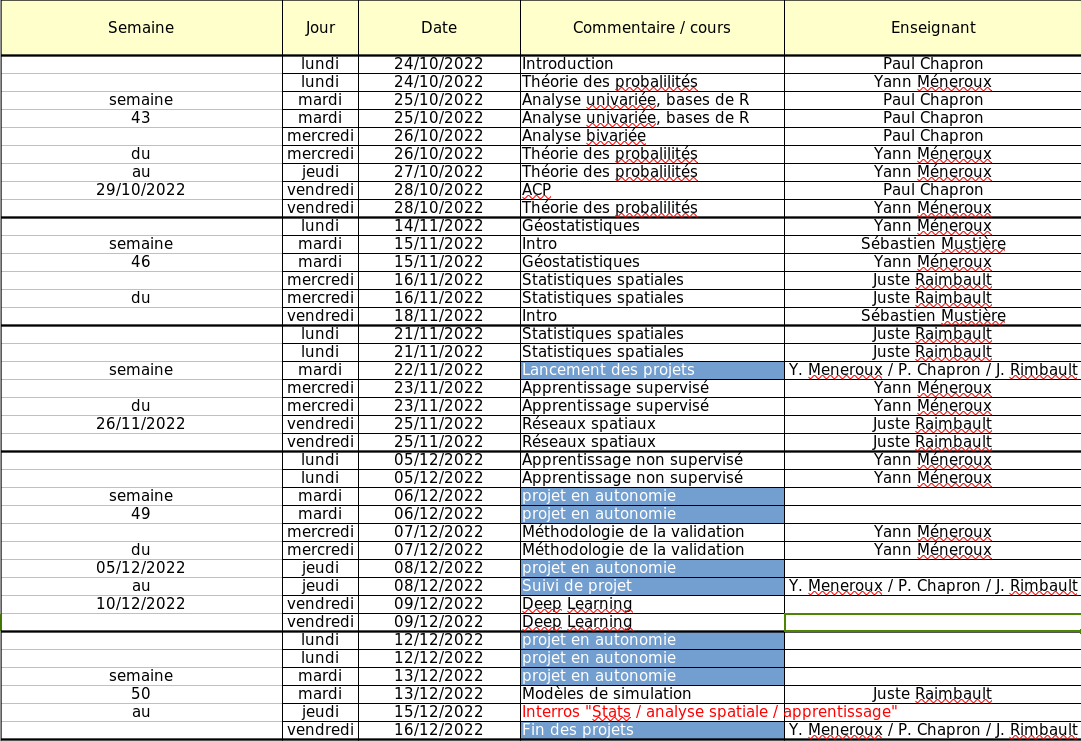
\includegraphics[width=\textwidth,keepaspectratio]{img/agenda2022.png}

\end{frame}








\begin{frame}
\frametitle{Tropes de la statistique}


Pendant la WW2, la Royal Air Force  voulait blinder ses avions contre la flotte et la DCA allemande. Blinder tout l'appareil est impossible car trop lourd. 

\alert{Où} blinder les avions ? 


On collecte des données : la localisation impacts de shrapnels  et de balles des avions \alert{rentrés} à la base en Angleterre. 
\end{frame}





\section{Tropes de la statistique}


\begin{frame}
\frametitle{L'avion}

\centering
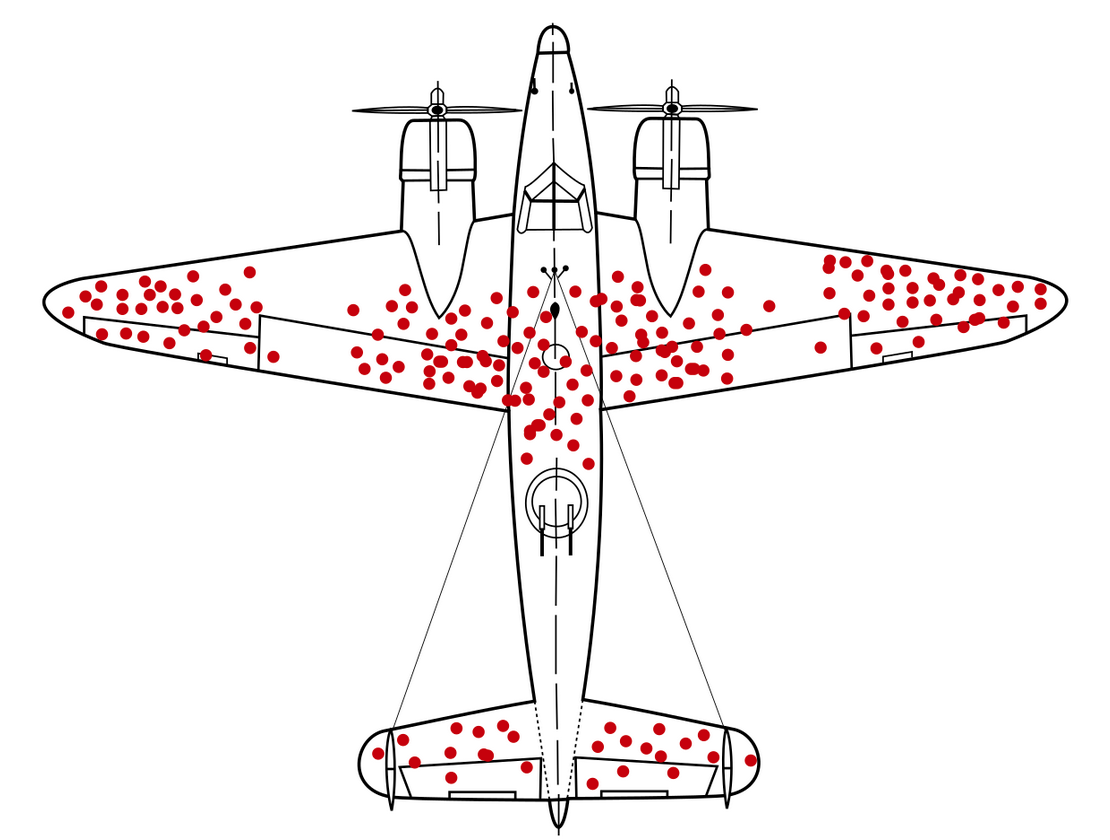
\includegraphics[width=\textwidth,keepaspectratio]{img/plane.png}





\end{frame}




\begin{frame}
\frametitle{L'avion anglais de la WW2}



$\rightarrow$ il faut blinder l'arrière et les ailes ! 

Mais ... 
\pause
il faut prendre en compte le \emph{\alert{biais du survivant} }

\pause

Les données proviennent d'avions qui sont \alert{rentrés} à la base.  
Ceux qui ont été touchés gravement ont péri, leurs impacts ne sont \alert{pas} dans les données.

Hypothèse :  les impacts sont uniformes sur les avions, \alert{mais} les avions rentrés le sont peut-être du fait que les impacts ont causé peu de dommages sur l'avion, leur permettant de rentrer.

\end{frame}

\begin{frame}
\frametitle{L'avion anglais de la WW2}


$\rightarrow$ il faut blinder le cockpit et les moteurs.

Ce qu'ils ont fait, avec succès (beaucoup moins de pertes).


\centering
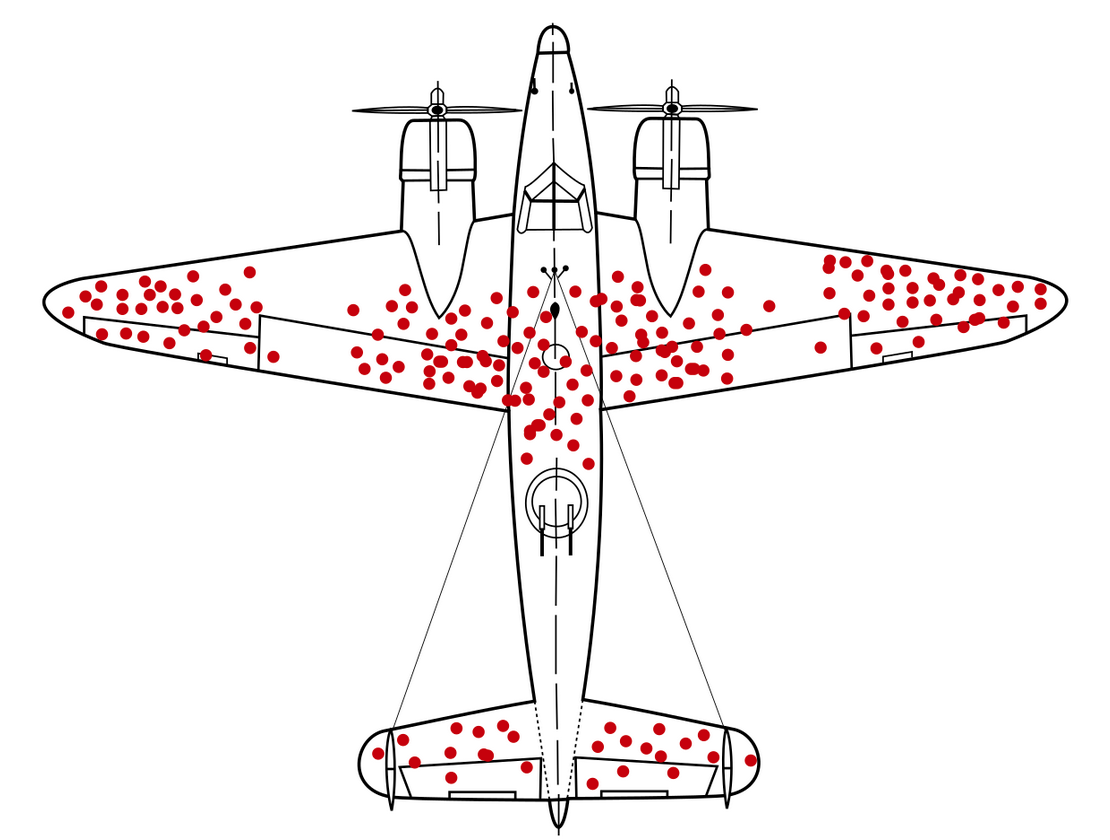
\includegraphics[width=0.7\textwidth,keepaspectratio]{img/plane.png}


\end{frame}

\begin{frame}
\frametitle{Spurious correlations}



\centering
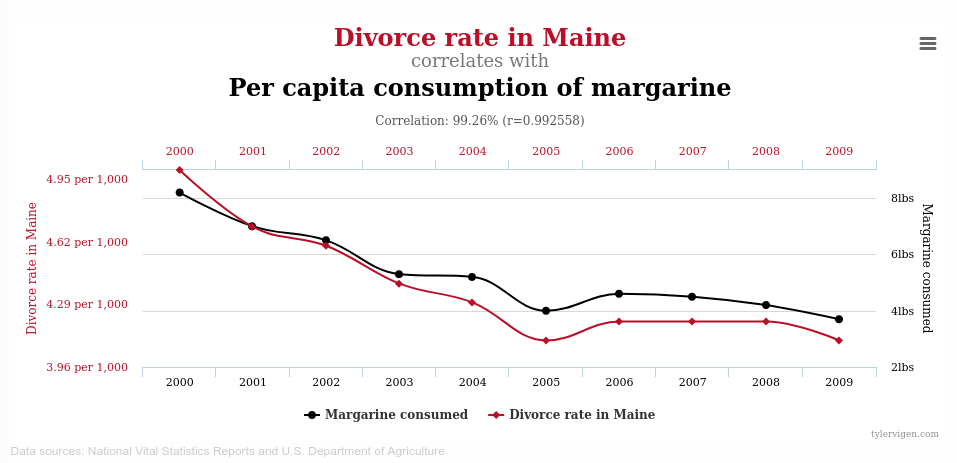
\includegraphics[width=0.8\textwidth,keepaspectratio]{img/spurious_corr.png}
\vfill
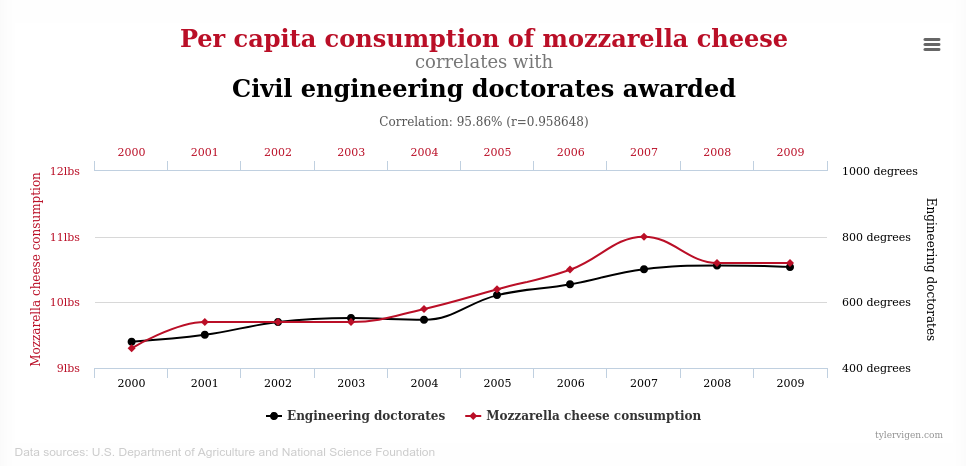
\includegraphics[width=0.8\textwidth,keepaspectratio]{img/spurious_corr2.png}

\end{frame}


\begin{frame}
\frametitle{Les "chiffres"}


Sur les mêmes chiffres du bilan d’une entreprise en 2013 et 2014

    \begin{itemize} 
    \item Mme. AAA : «tous les salaires ont baissé de 10\%»
    \item M. BBB : «le salaire moyen a augmenté d’environ 18\%»
  \end{itemize}
  
\begin{table}[]
\begin{tabular}{|l|r|r|}
\hline
\textbf{} & \textbf{Ouvriers} & \textbf{Cadres} \\ \hline
2013      & effectif : 500    & effectif : 100  \\ \hline
          & salaire : 1300    & salaire :2200   \\ \hline
2014      & effectif : 200    & effectif : 400  \\ \hline
          & salaire :1170     & salaire : 1980  \\ \hline
\end{tabular}
\end{table}

\end{frame}


\begin{frame}
\frametitle{La fragilité  de la moyenne}


Salaire moyen en 2020 EQTP (hors Mayotte) : 2518€ 

\centering
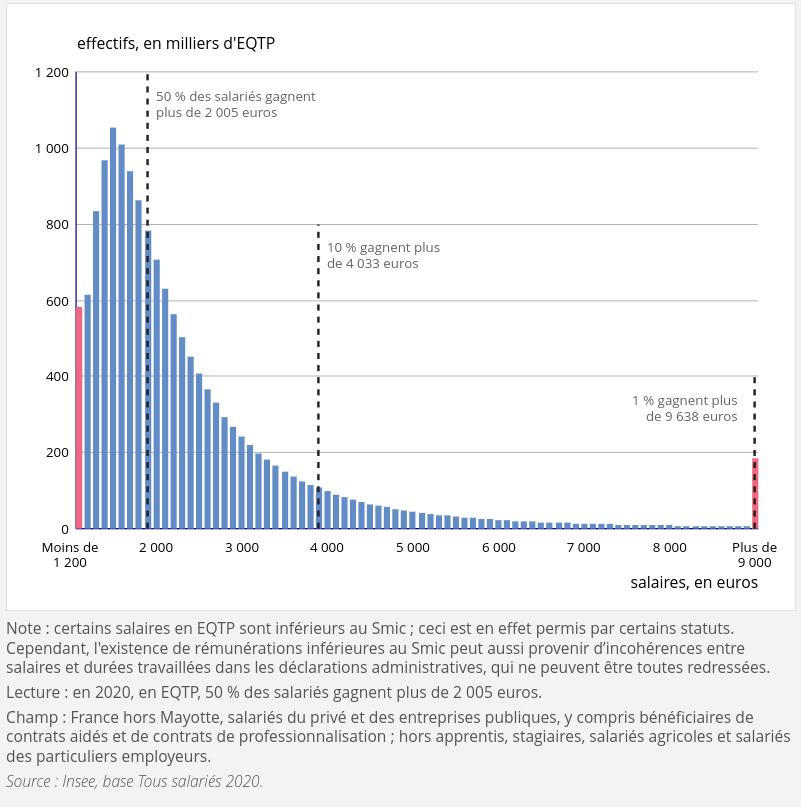
\includegraphics[width=0.7\textwidth,keepaspectratio]{img/salaire.png}


\end{frame}



\begin{frame}
\frametitle{La fragilité de la moyenne}

«Quand les distributions sont \alert{unimodales et symétriques}, tout va bien.» \\

Sinon, agir avec précaution !  

\end{frame}


\section{Représenter les données}


\begin{frame}
\frametitle{La première chose à faire}

Toujours «jeter un oeil» aux données.  A fortiori si elles sont spatiales ! 

\begin{itemize}
 \item identification des tendances, des motifs
 \item complétude 
 \item outliers
\end{itemize}

Visualiser \alert{avant} : analyse visuelle exploratoire  et \\ 
Visulaiser  \alert{après}  :restituition/diffusion  des résultats des traitements 

\end{frame}





\begin{frame}
\frametitle{Mais il faut le faire bien}

\alert{Toujours}

\begin{itemize}
  \item étiqueter les axes (unités)
  \item fournir une légende complète 
  \item choisir des classes de valeurs et de couleurs sensées
  \item penser au support de diffusion 
\end{itemize}

\end{frame}


\begin{frame}
\frametitle{Critère de réussite}

\alert{«Self explanatory»} : Si on se demande quoi voir ou comment lire, c'est raté. Si c'est moche, trop petit, peu lisible, idem.


\vspace{1cm}


$\implies$Faites simple 

\end{frame}



\section{Exemples réussis}




\begin{frame}
\centering
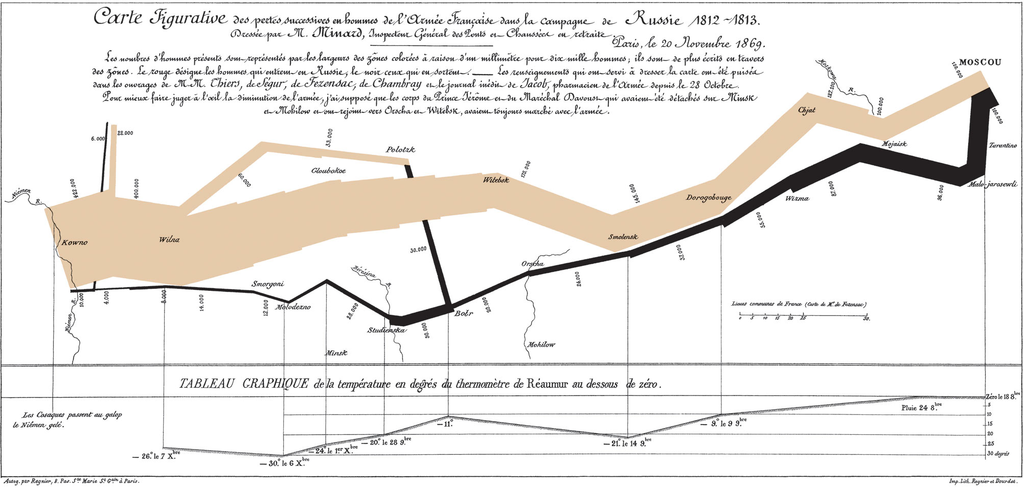
\includegraphics[width=\textwidth,keepaspectratio]{img/minard.png}
\end{frame}



\begin{frame}
\centering
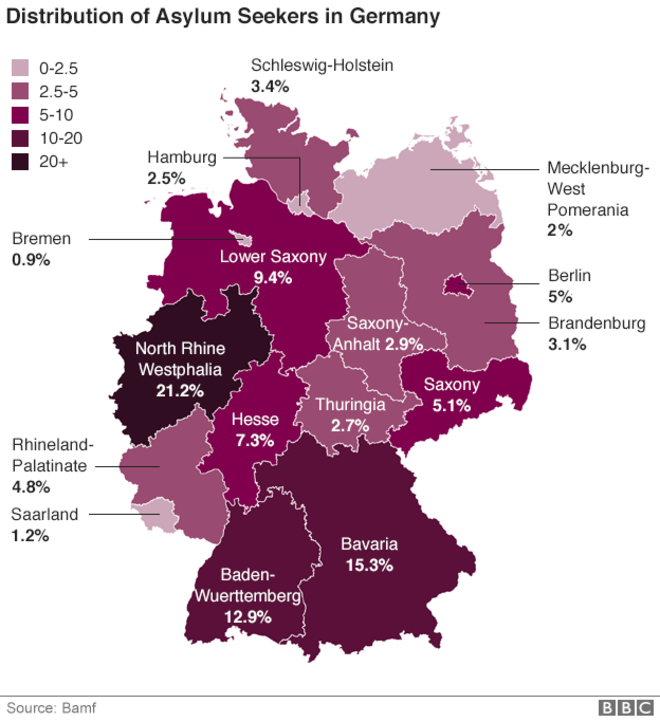
\includegraphics[width=\textwidth,keepaspectratio]{img/bon_exemple.png}
\end{frame}


\begin{frame}
\centering
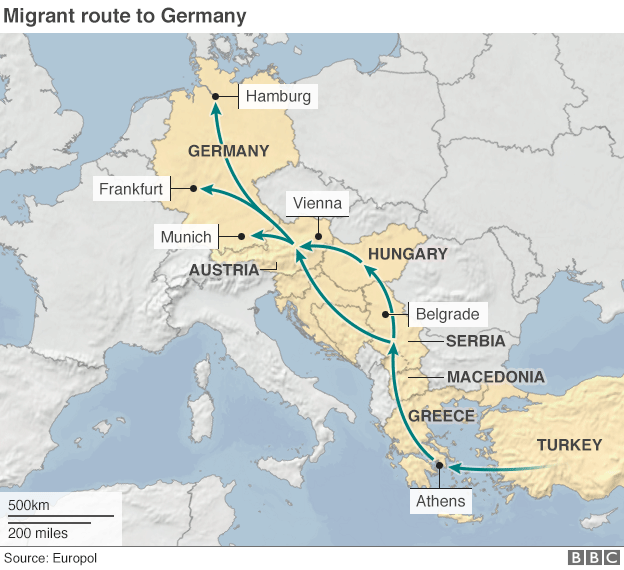
\includegraphics[width=\textwidth,keepaspectratio]{img/bon_exemple2.png}
\end{frame}

\begin{frame}
\centering
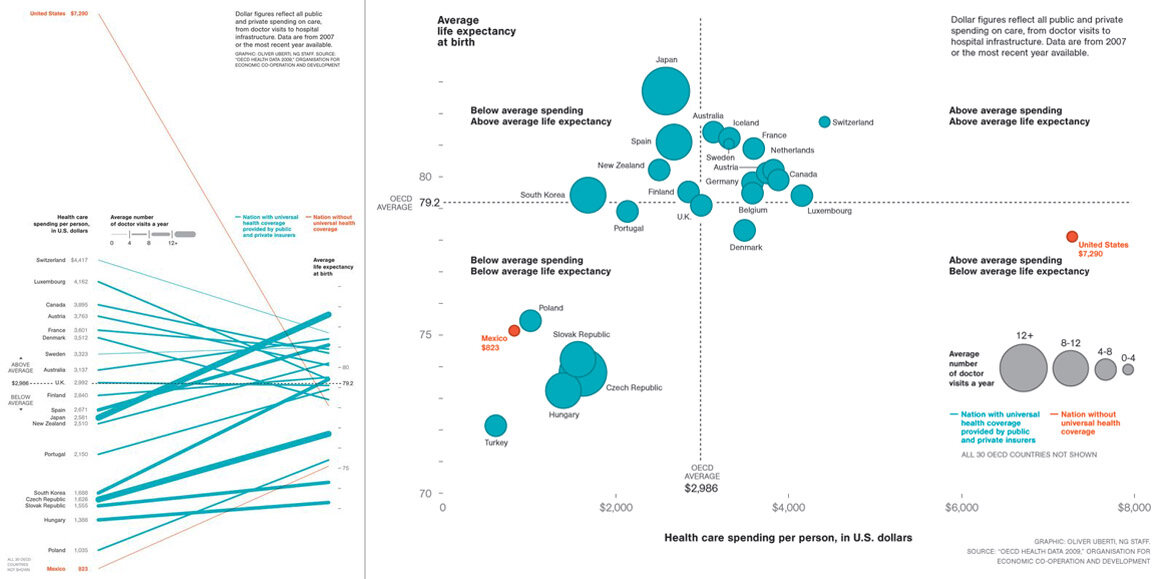
\includegraphics[width=\textwidth,keepaspectratio]{img/bon_exemple3.jpg}
\end{frame}


\begin{frame}
\centering
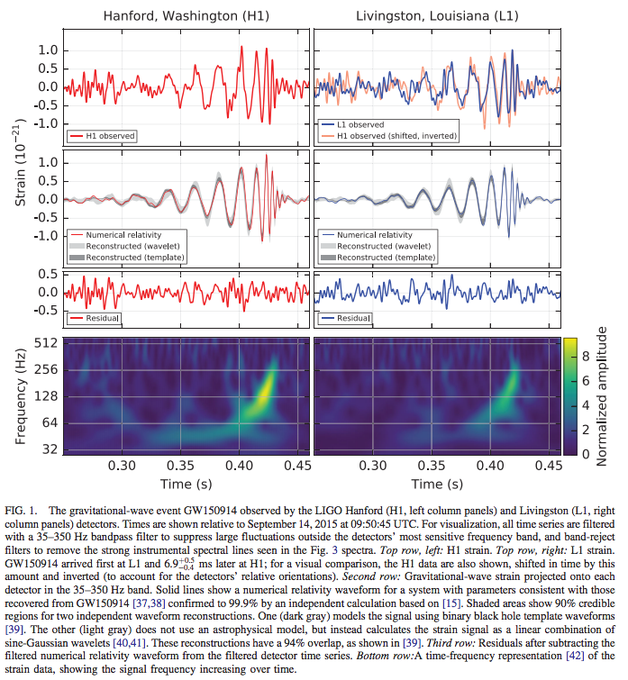
\includegraphics[width=0.75\textwidth,keepaspectratio]{img/bon_exemple4.png}

\tiny{source : \url{https://twitter.com/PhysRevLett/status/697815592062074881} }
\end{frame}




\begin{frame}
\centering
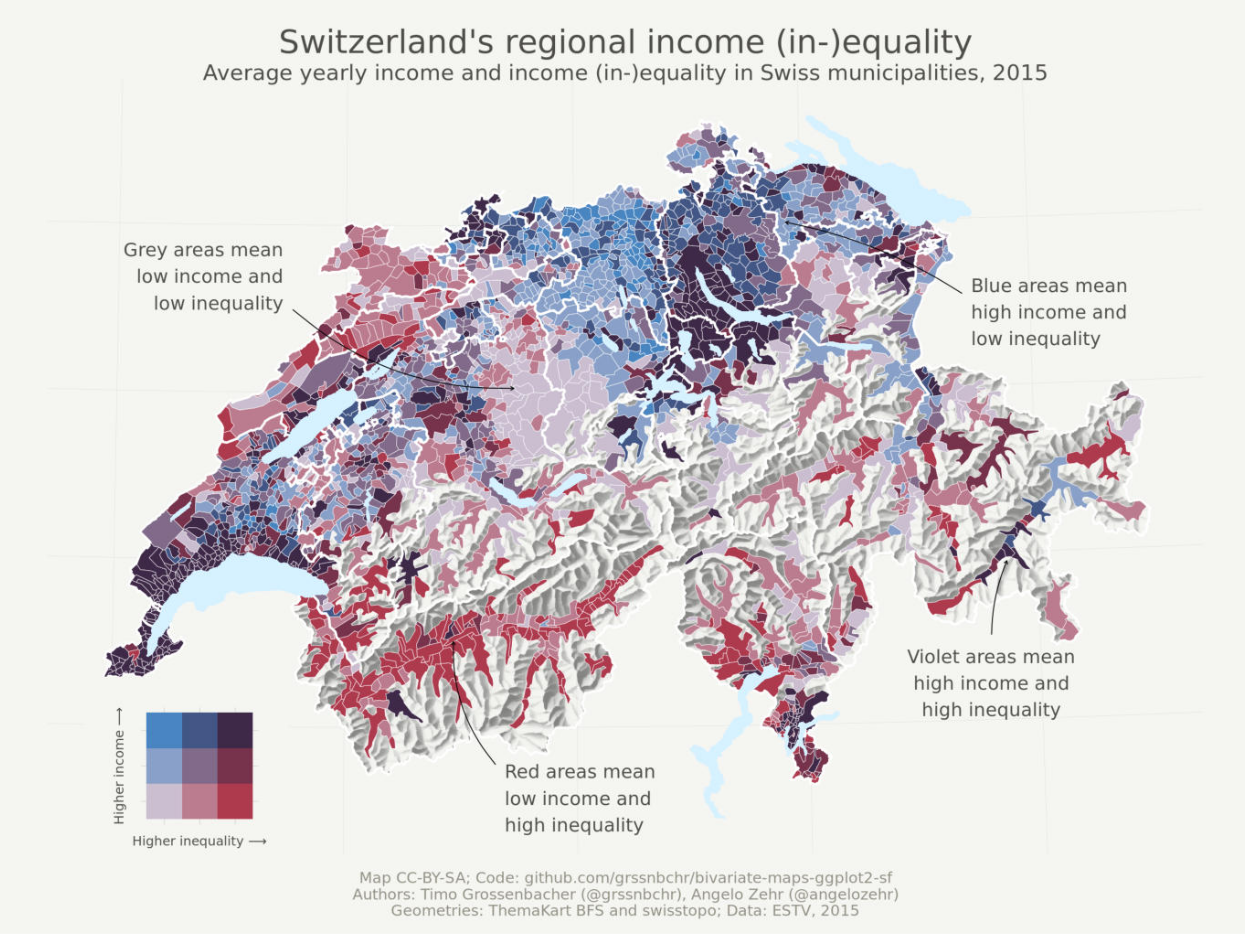
\includegraphics[width=\textwidth,keepaspectratio]{img/carto_suisse.png}
\end{frame}



\begin{frame}
\centering
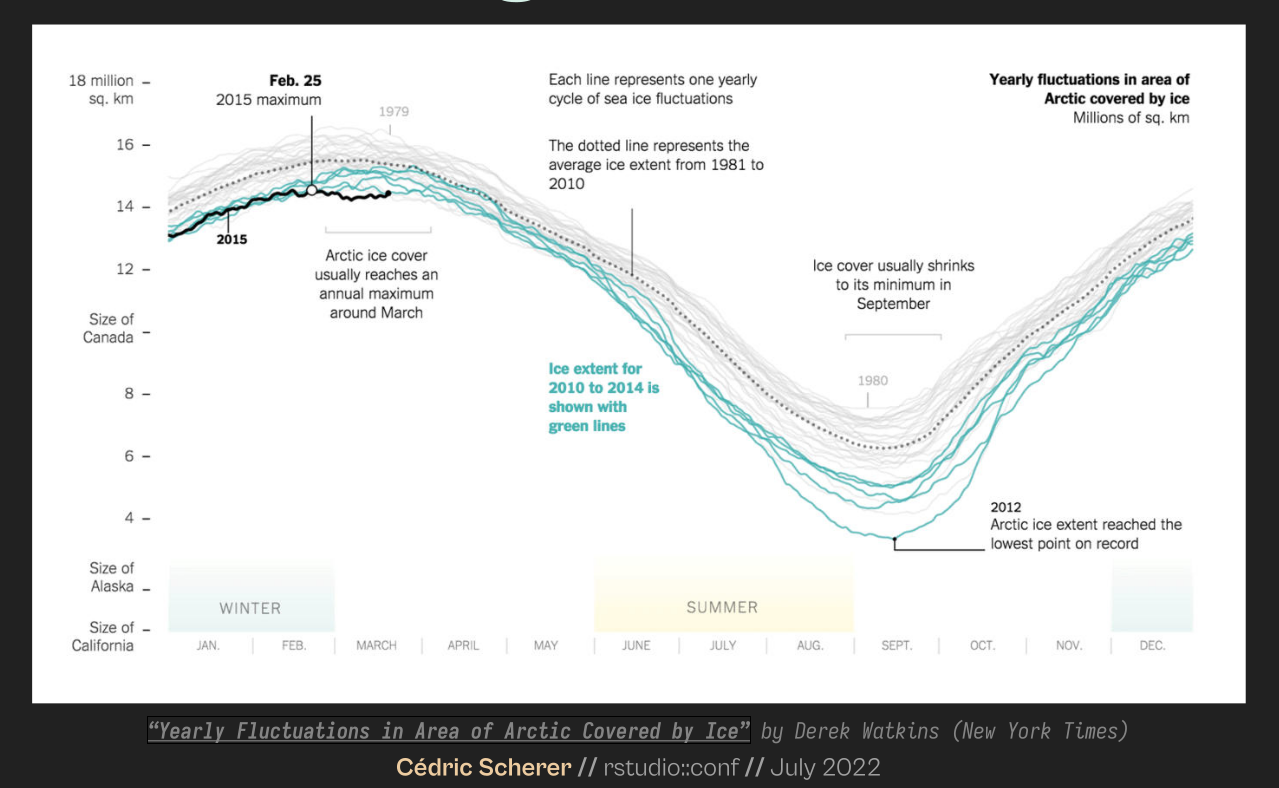
\includegraphics[width=\textwidth,keepaspectratio]{img/good_viz.png}

\end{frame}






\section{Musées des horreurs}



 \begin{frame}\centering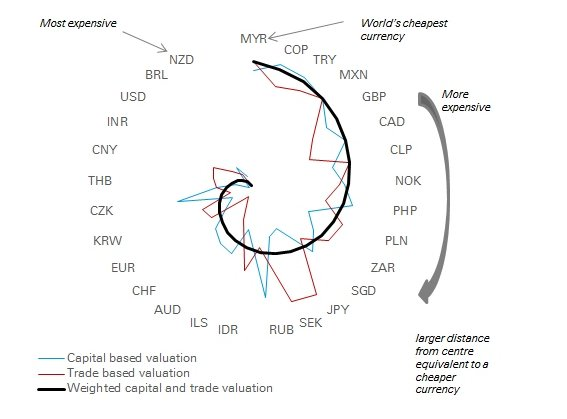
\includegraphics[width=\textwidth,keepaspectratio]{graphcrimes/DLckOPNWAAA0cy4.jpeg}\end{frame}
 \begin{frame}\centering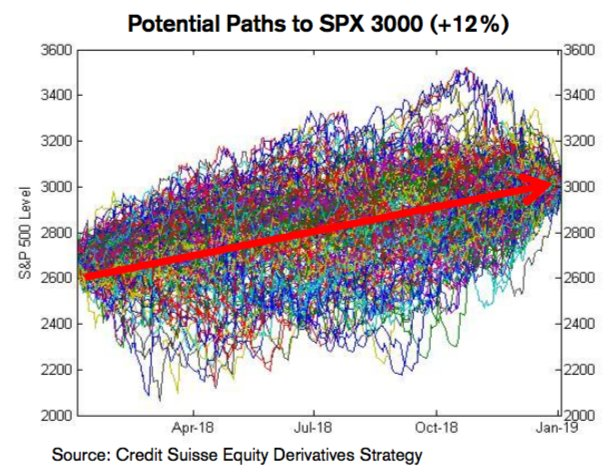
\includegraphics[width=\textwidth,keepaspectratio]{graphcrimes/DTyVpdiV4AAnVov.jpeg}\end{frame}
 \begin{frame}\centering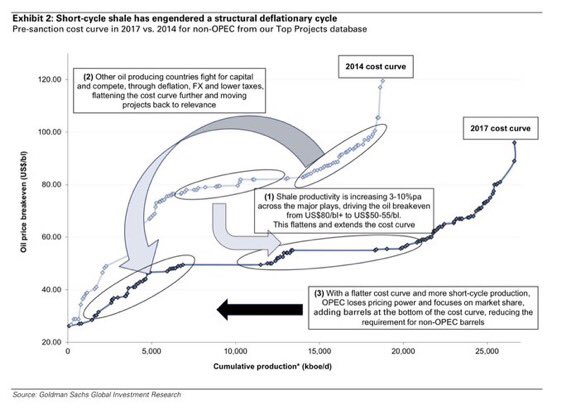
\includegraphics[width=\textwidth,keepaspectratio]{graphcrimes/DXfpXfmX0AAgMrS.jpeg}\end{frame}
 \begin{frame}\centering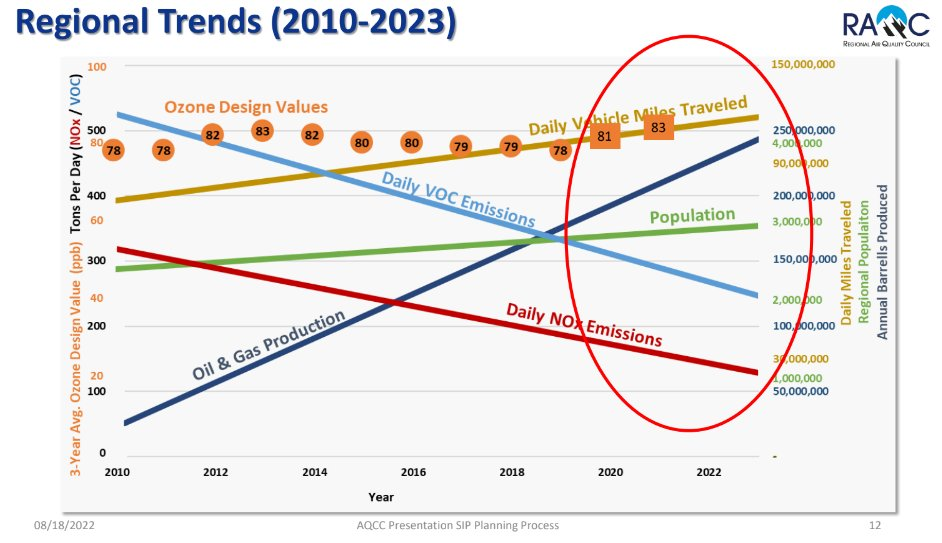
\includegraphics[width=\textwidth,keepaspectratio]{graphcrimes/FaYCYQFWQAAm3DB.jpeg}\end{frame}
 \begin{frame}\centering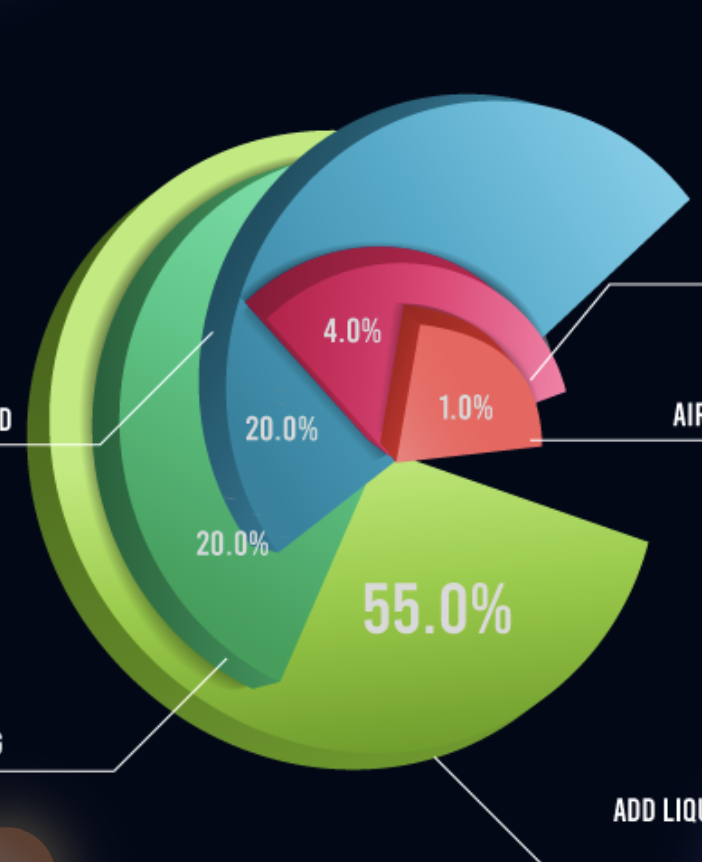
\includegraphics[width=0.7\textwidth,keepaspectratio]{graphcrimes/FN8ErPaXwAIEdO3.png}\end{frame}
 \begin{frame}\centering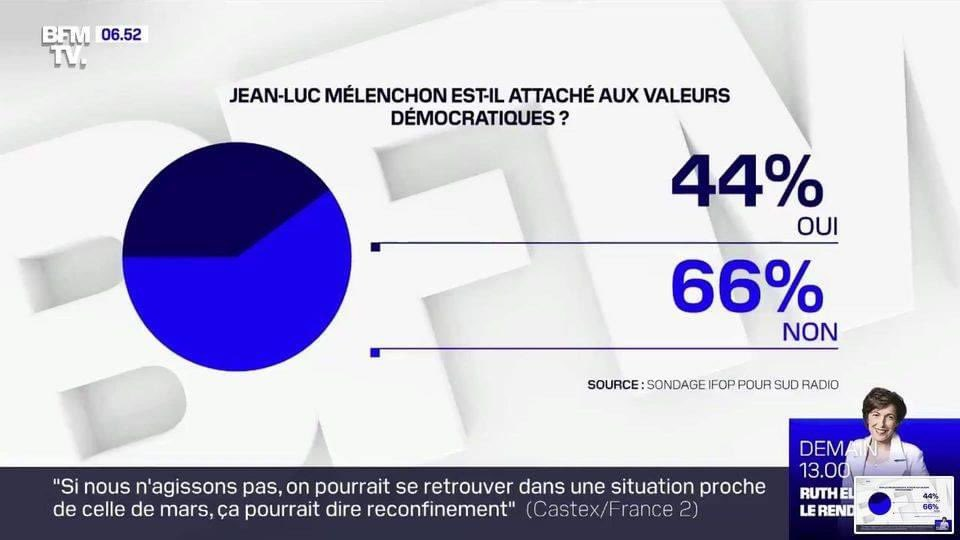
\includegraphics[width=\textwidth,keepaspectratio]{graphcrimes/FQHLjS5XwAY4pp1.jpeg}\end{frame}
 \begin{frame}\centering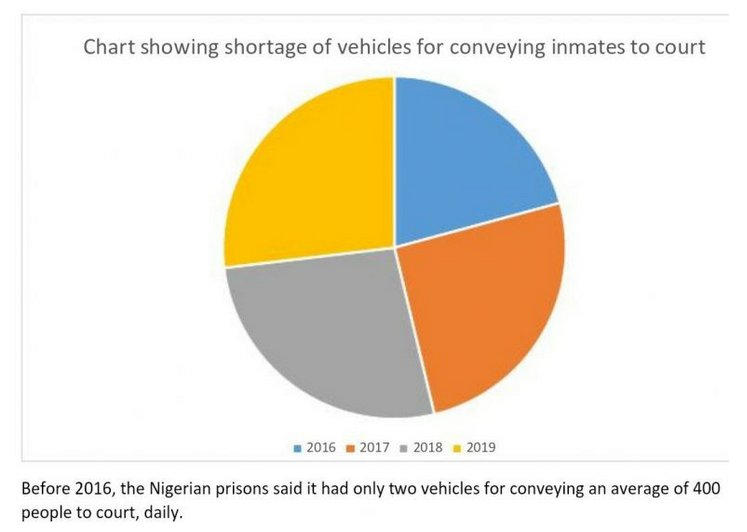
\includegraphics[width=\textwidth,keepaspectratio]{graphcrimes/FRSll9GWYAMyYZR.jpeg}\end{frame}
 \begin{frame}\centering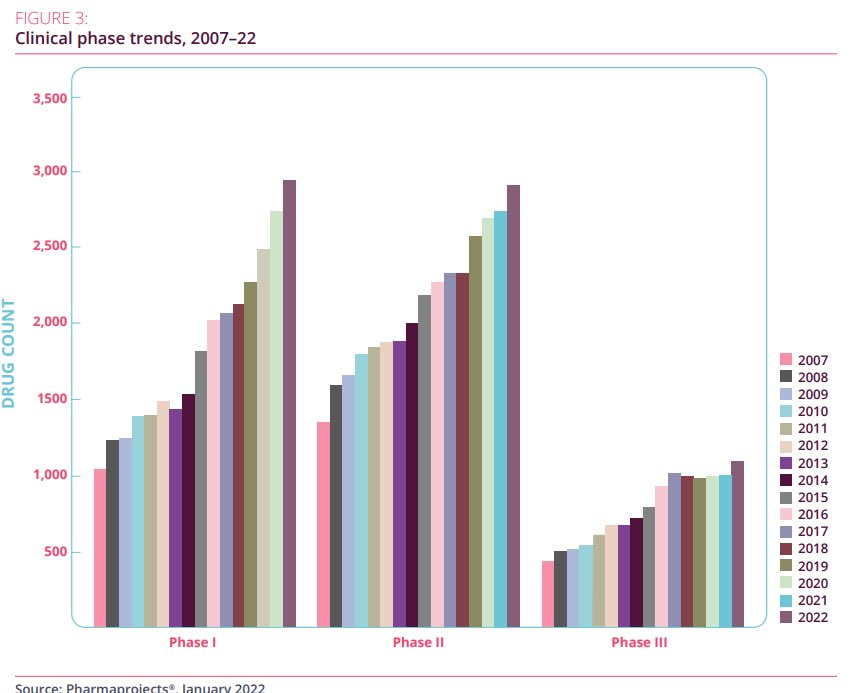
\includegraphics[width=\textwidth,keepaspectratio]{graphcrimes/FRUFGM4WUAEq35D.jpeg}\end{frame}
 \begin{frame}\centering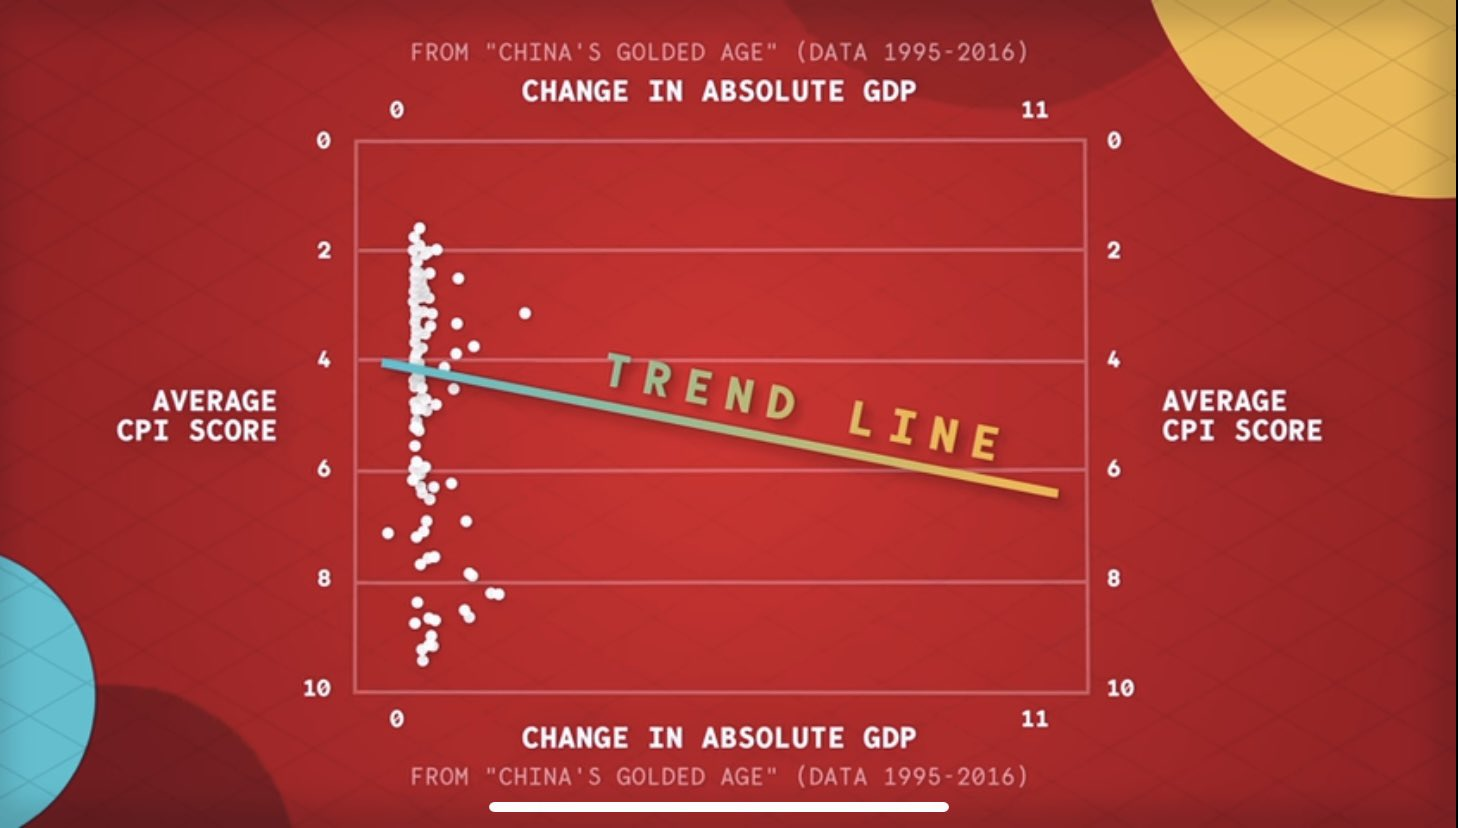
\includegraphics[width=\textwidth,keepaspectratio]{graphcrimes/FSiH5AwXoAA8w23.jpeg}\end{frame}
 \begin{frame}\centering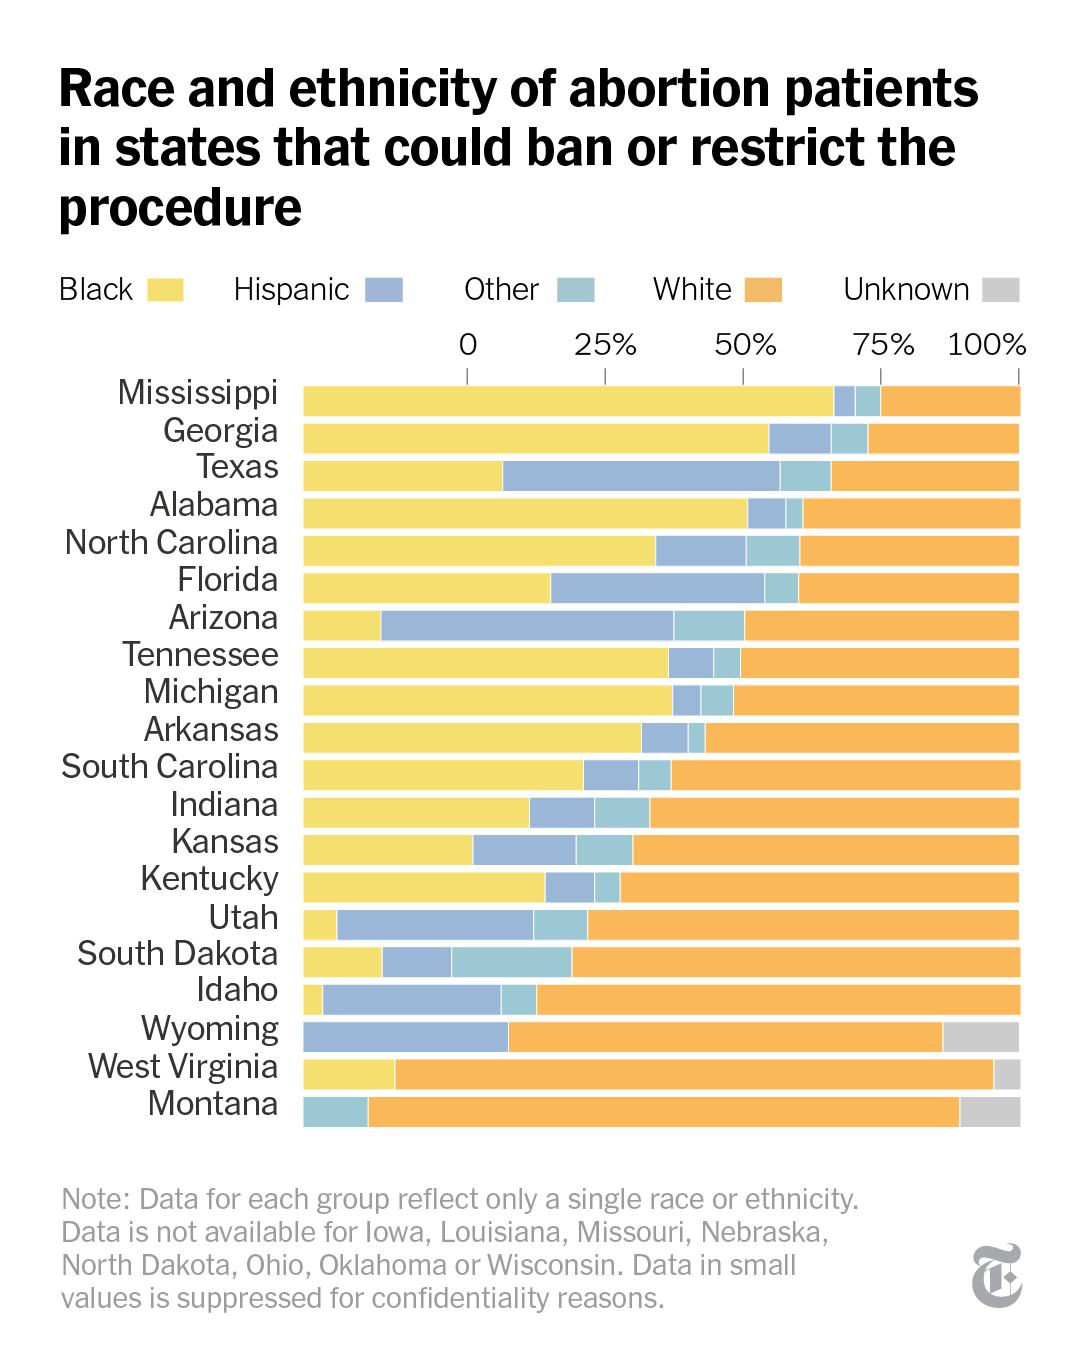
\includegraphics[width=0.7\textwidth,keepaspectratio]{graphcrimes/FSP19zkXIAAiUmi.png}\end{frame}
 \begin{frame}\centering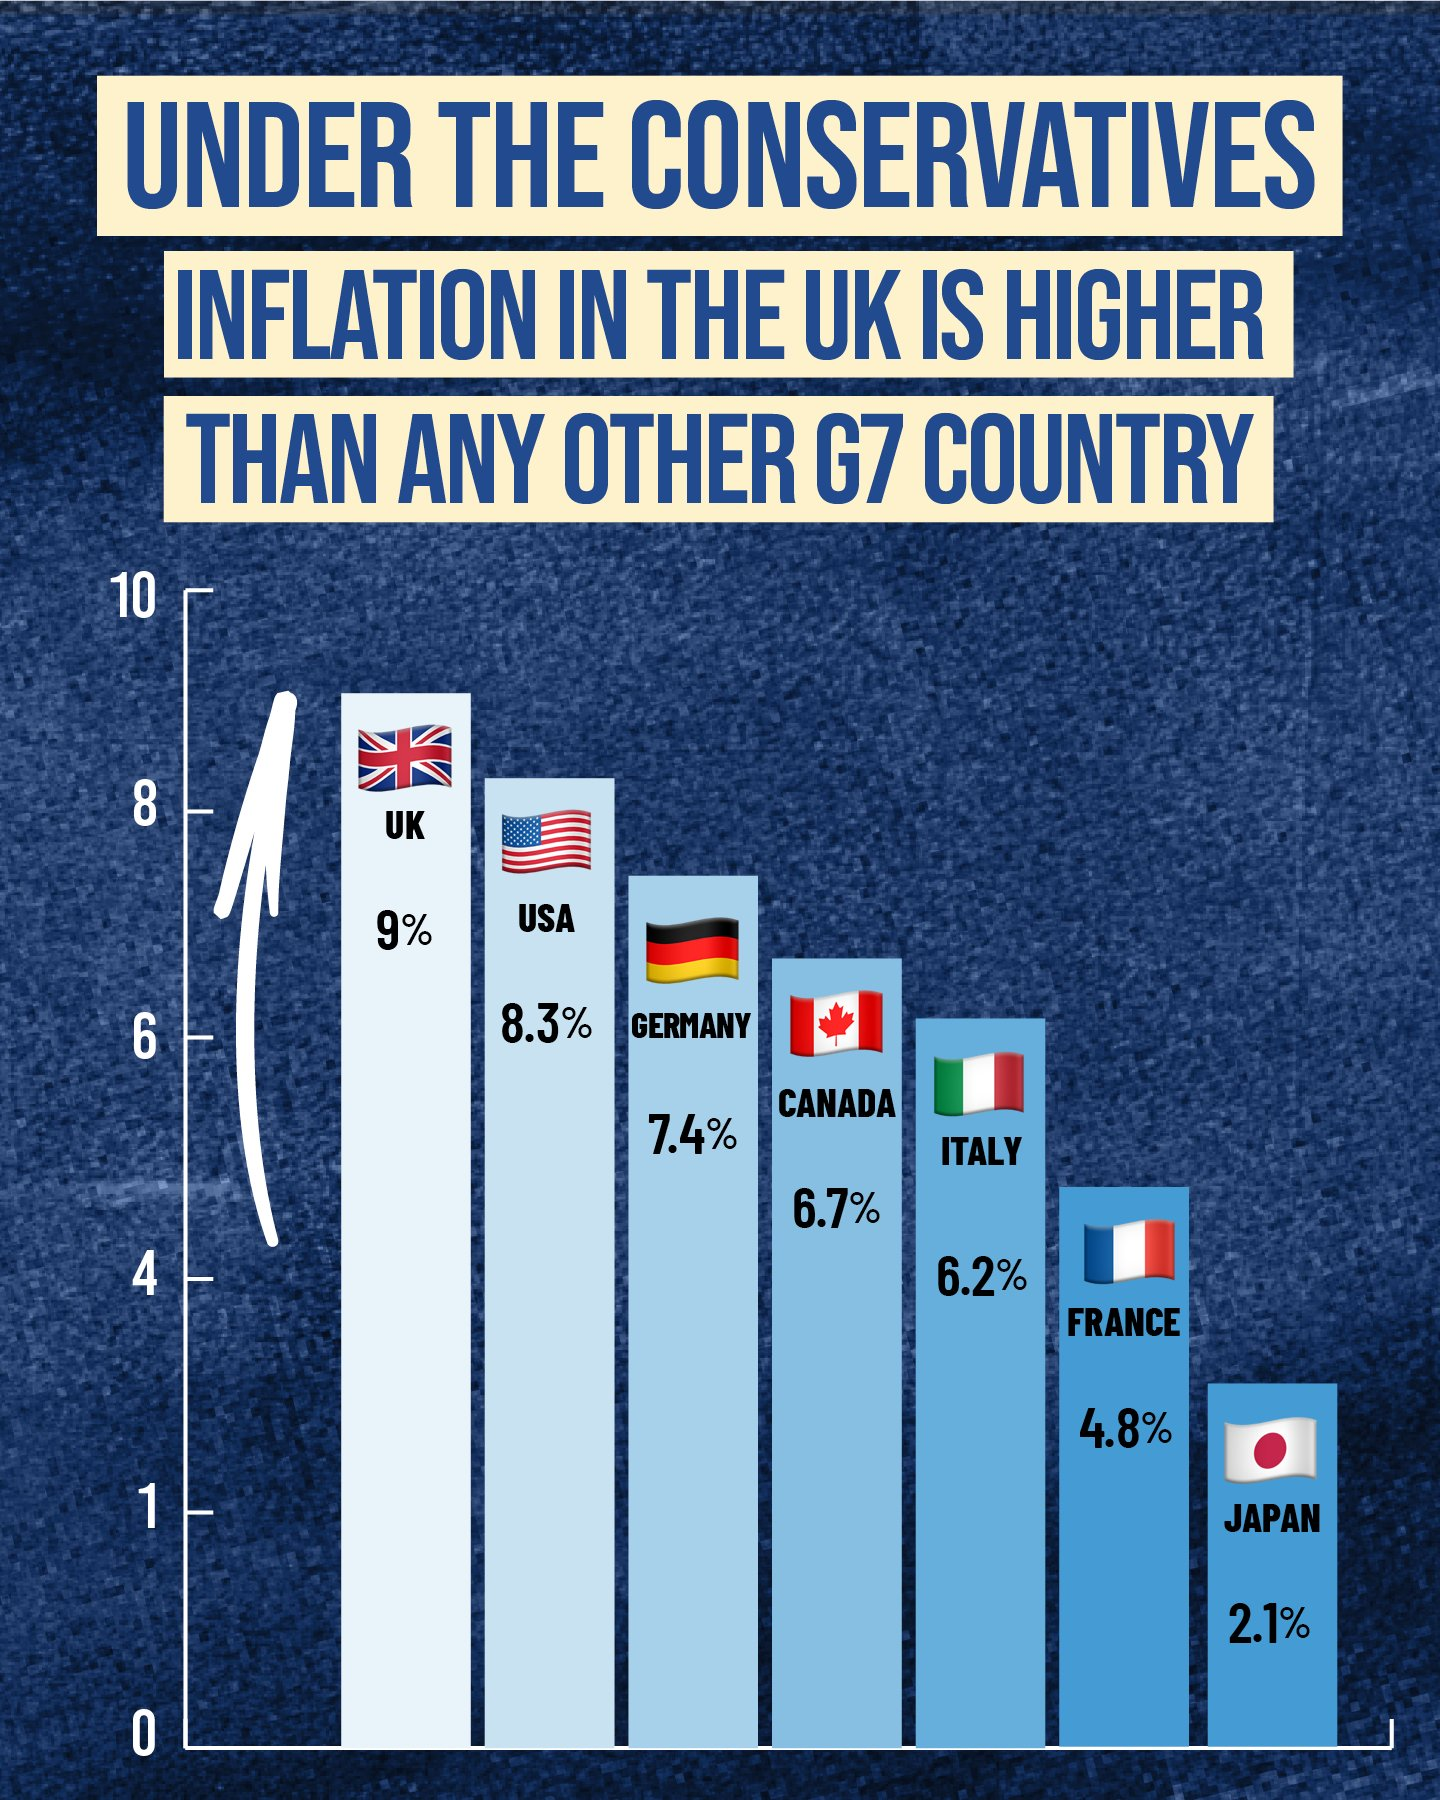
\includegraphics[width=0.7\textwidth,keepaspectratio]{graphcrimes/FTME9qxWQAIZLbe.jpeg}\end{frame}
 \begin{frame}\centering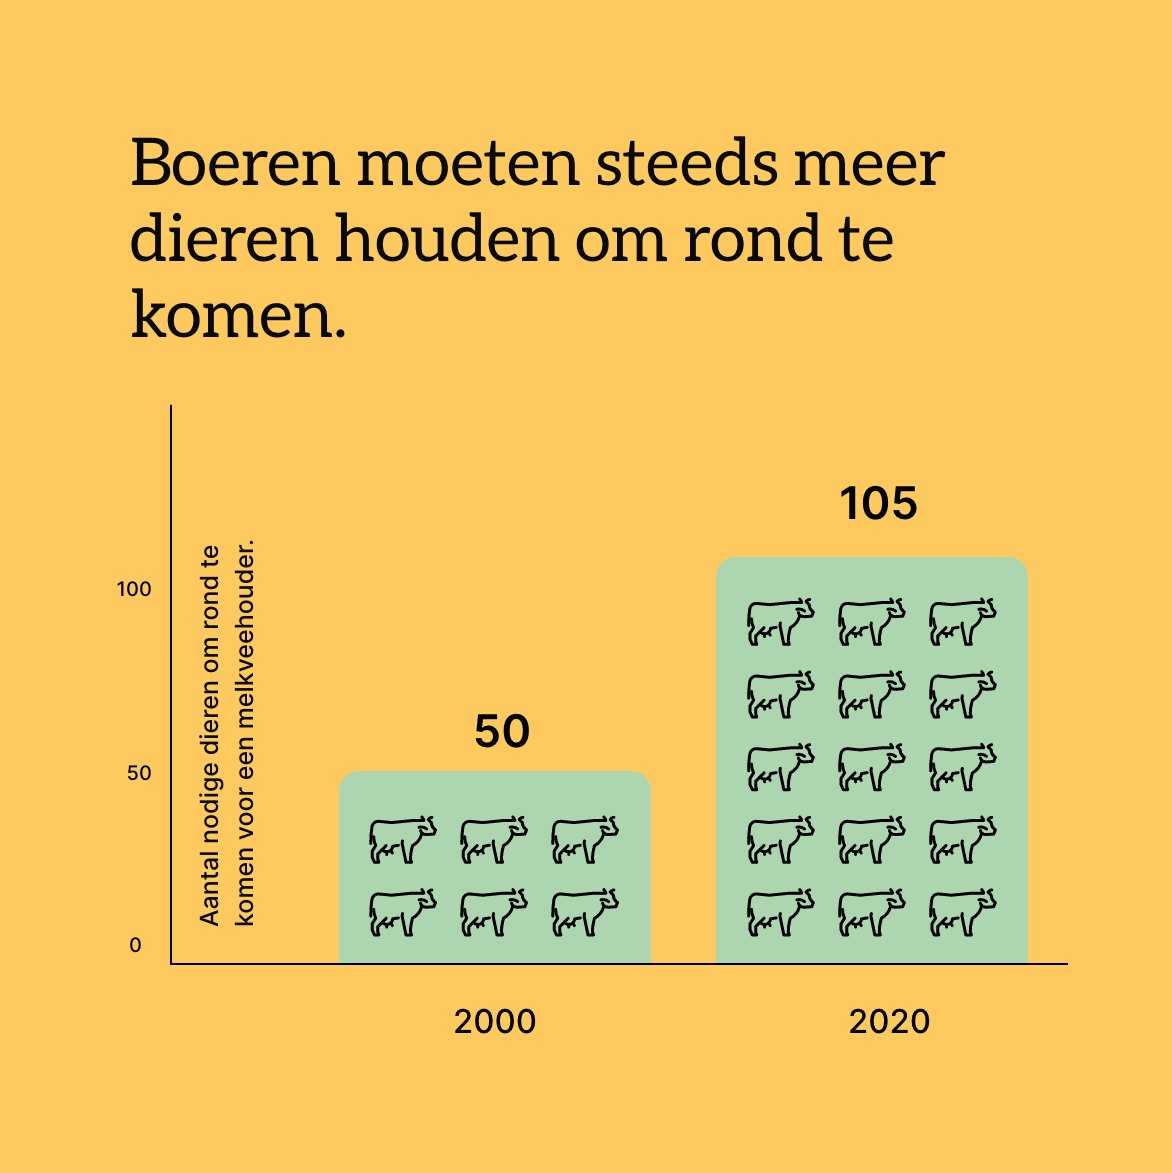
\includegraphics[width=0.9\textwidth,keepaspectratio]{graphcrimes/FVdSWe5XsAAYJGH.jpeg}\end{frame}
 \begin{frame}\centering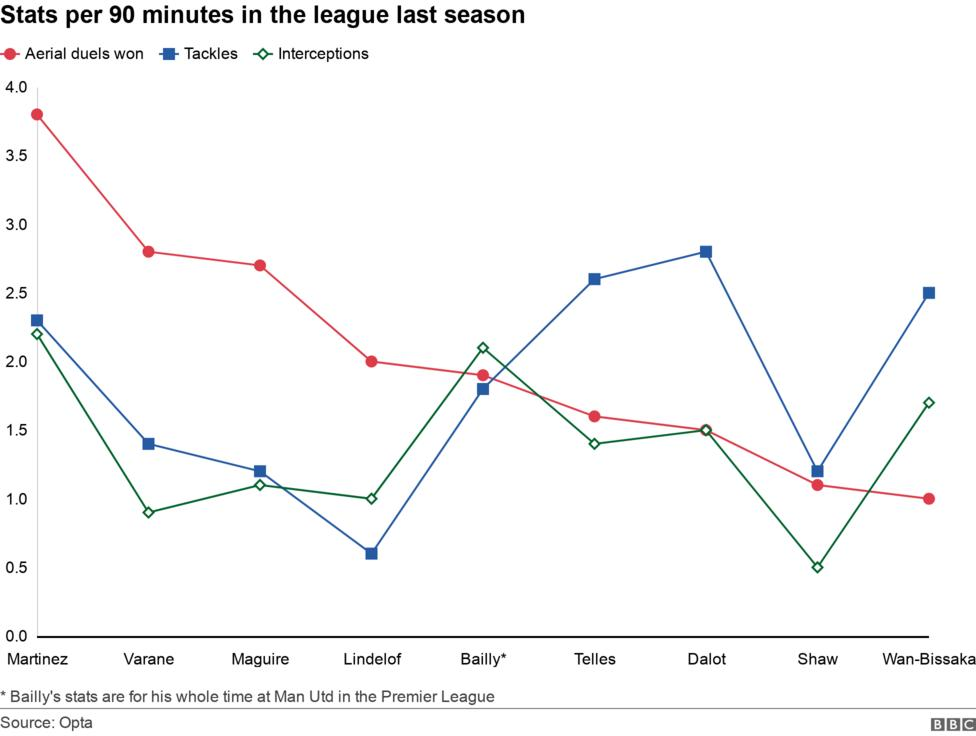
\includegraphics[width=\textwidth,keepaspectratio]{graphcrimes/FX7LWekXEAIr0lP.jpeg}\end{frame}
 \begin{frame}\centering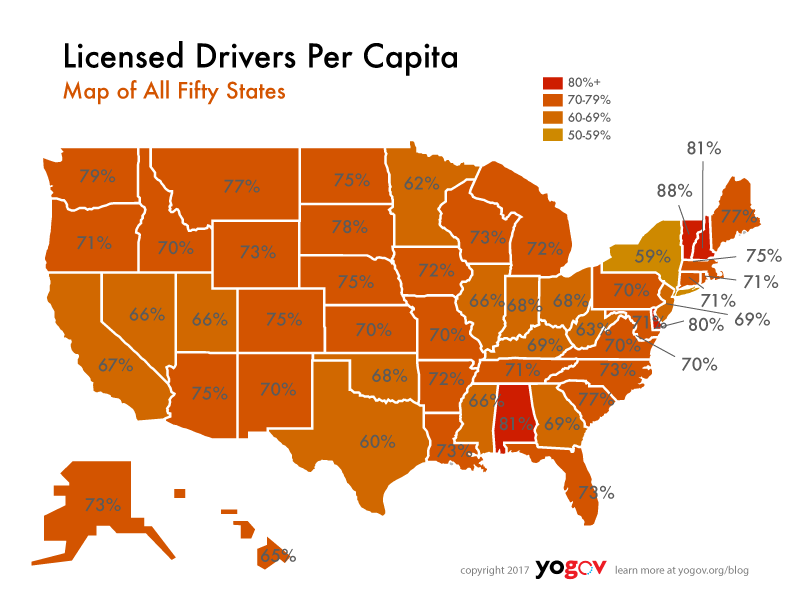
\includegraphics[width=\textwidth,keepaspectratio]{graphcrimes/FXBQtakXEAAFVc7.png}\end{frame}
 \begin{frame}\centering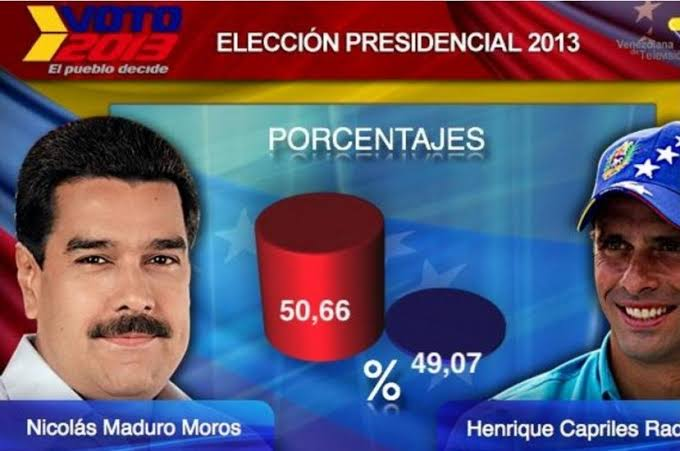
\includegraphics[width=\textwidth,keepaspectratio]{graphcrimes/FXz7CxPVQAAJVuL.jpeg}\end{frame}
 \begin{frame}\centering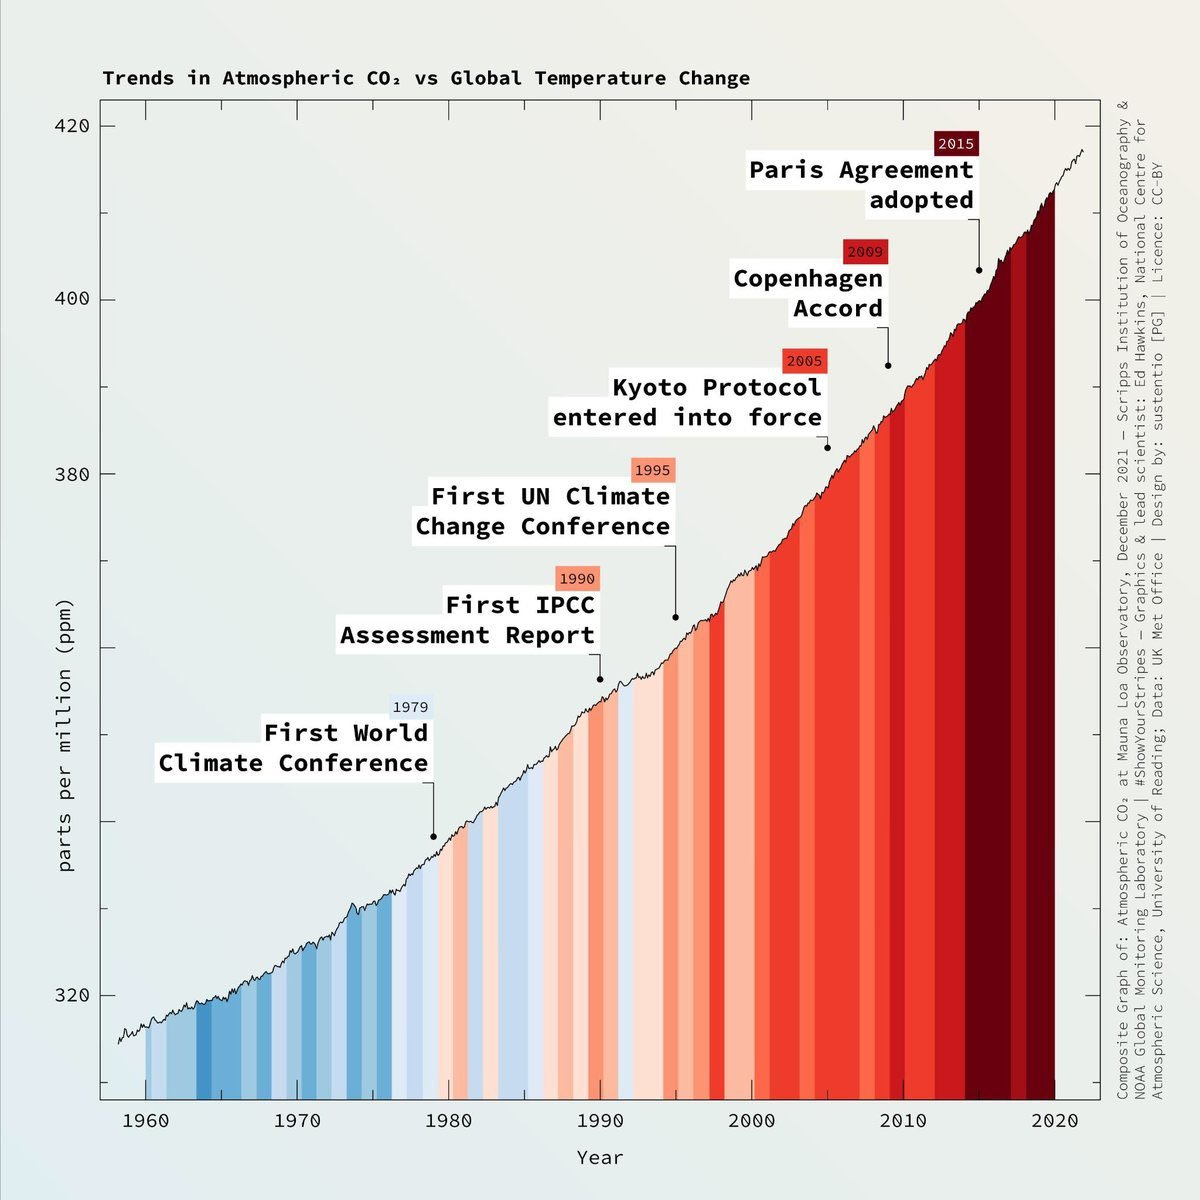
\includegraphics[width=0.9\textwidth,keepaspectratio]{graphcrimes/FYi_zJZVEAAxFW9.jpeg}\end{frame}
 \begin{frame}\centering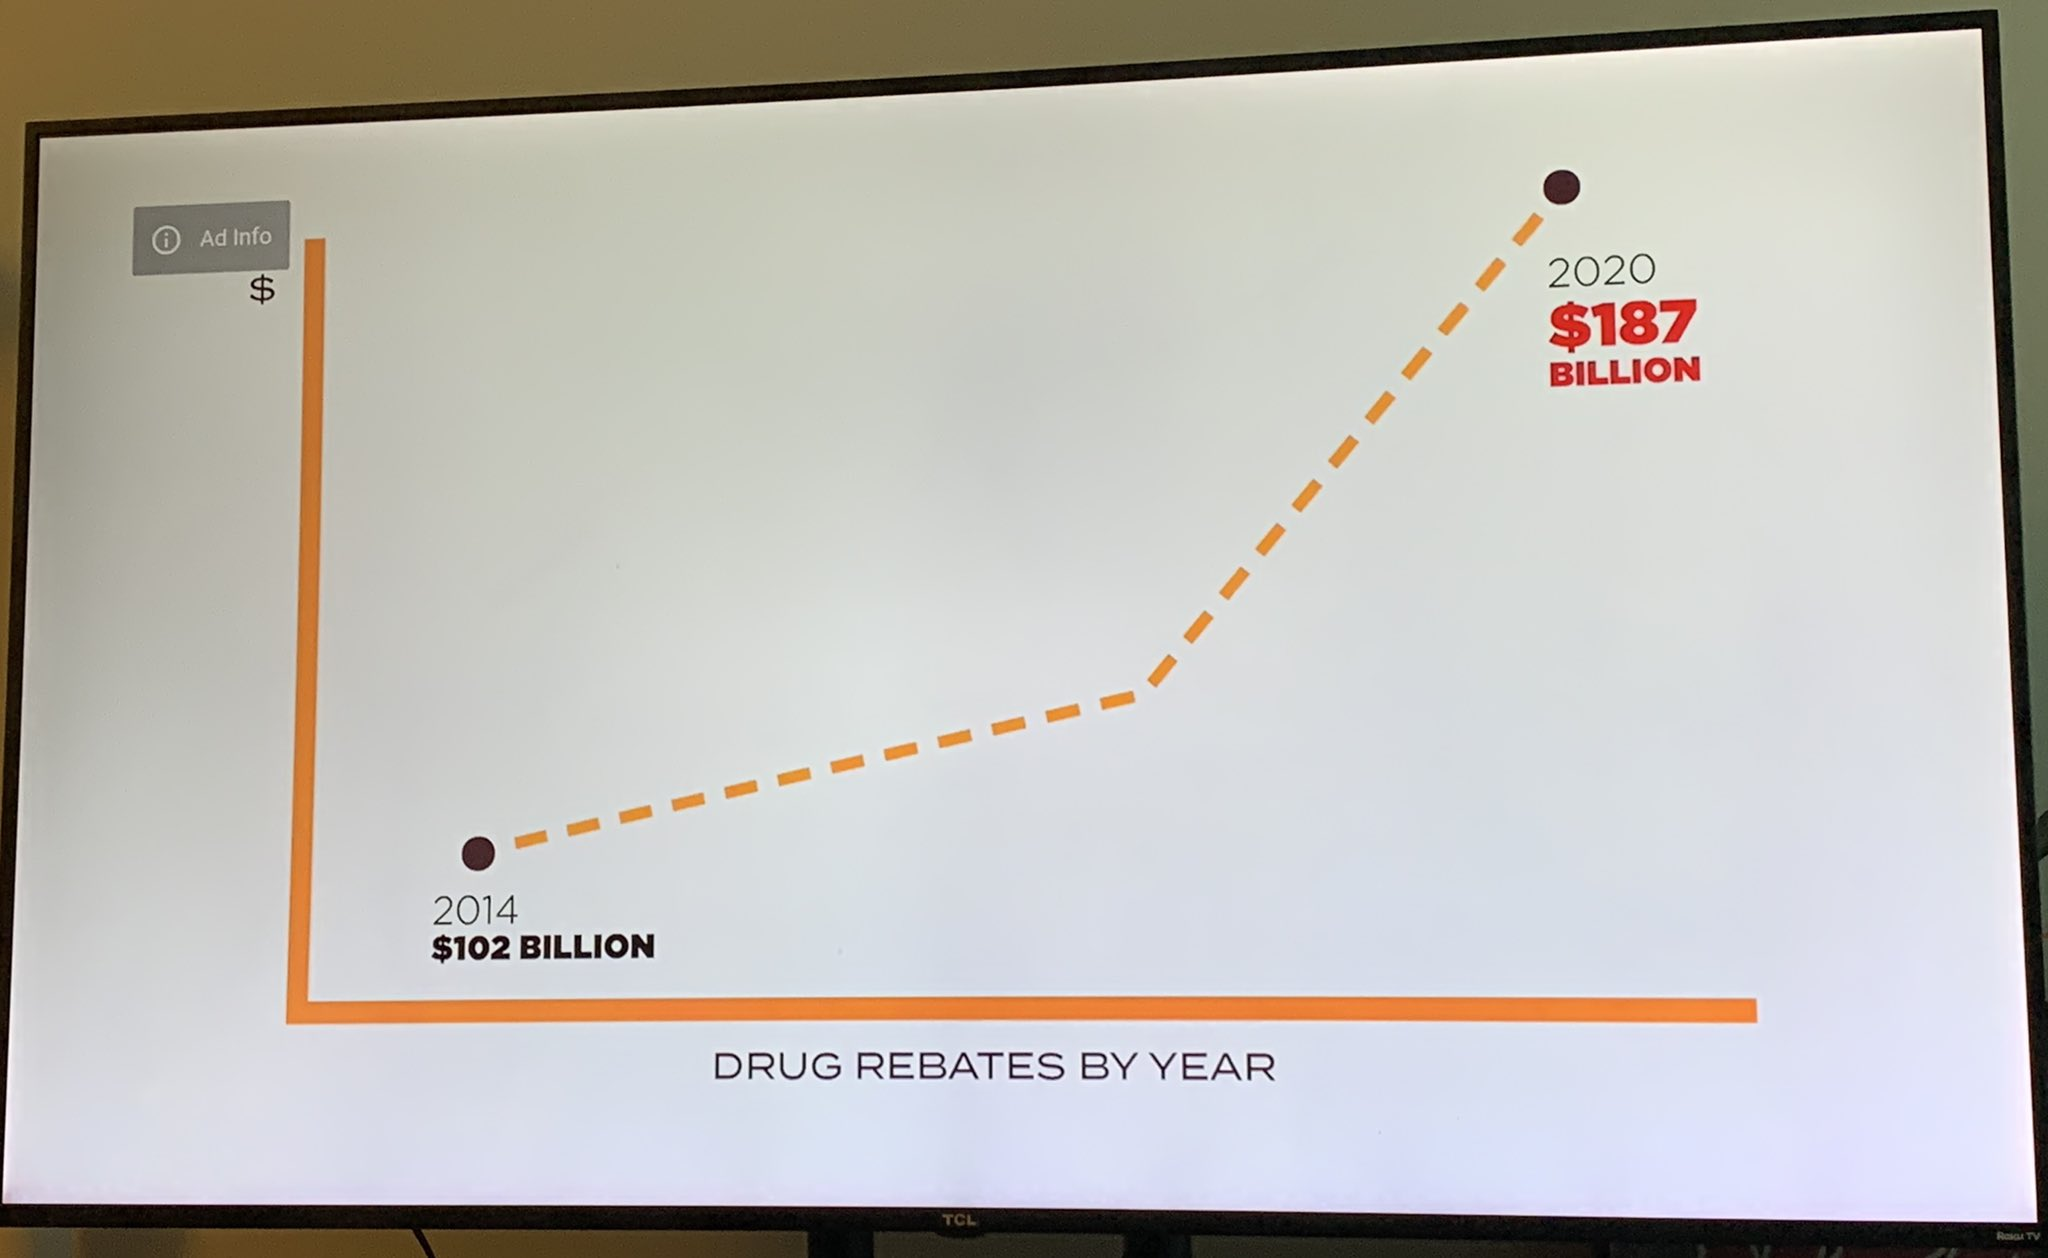
\includegraphics[width=\textwidth,keepaspectratio]{graphcrimes/FZwXuJjX0AEhyz-.jpeg}\end{frame}




\end{document}

